\documentclass[11pt]{article}
\usepackage[utf8]{inputenc}
%\usepackage[T1]{fontenc}
\usepackage{amssymb}
\usepackage{amsmath}
\usepackage{enumerate}
\usepackage{fullpage}
\usepackage{polski}  
\usepackage{indentfirst} 
\usepackage[pdftex]{graphicx}
\usepackage{multirow}
\usepackage{placeins}

\author{Łukasz Dubiel}

\begin{document}
\section{Opracowywanie wyników}
Do obliczeń bierzemy pierwsze maksimum
$$ x = 4 mm \quad \Delta x = 0,5 mm \quad \frac{\Delta x}{x} = 12,5\% $$
$$ l = 785mm \quad \Delta l = 5mm \quad \frac{\Delta l}{l} = 0,6 \% $$
$$ \lambda = 633 nm \quad \Delta \lambda = 1 nm \quad \frac{\Delta \lambda}{\lambda} = 0,1 \%$$
gdzie $x$ to odległość od głównej wiązki, $l$ - odległość płaszczyzny ruchu fotodiody od szczeliny. 
Wzór $$ d = (2m + 1) \frac{\lambda}{2 \sin{\varphi}} \quad m = 1,2,3\ldots $$
$$ \sin{\varphi} = \frac{x}{\sqrt{x^2 + l^2}} $$ 
$$ d = (2m + 1) \frac{\lambda}{x} \sqrt{x^2 + l^2} $$
Ale możemy wykorzystać przybliżenie
$$ \sin{\varphi} \approx \tan{\varphi} = \frac{x}{l} $$ 
Dzięki czemu upraszcza się nam wzór 
$$ d = (2m+1) \frac{\lambda l }{x} $$
$$ d = 3 \frac{633 \cdot 10^{-9} \cdot 785 \cdot 10^{-3}}{4 \cdot 10^{-3}} = 124 \cdot 10^{-6} = 124\ \mu m $$

$$\frac{dd}{d} = \frac{dl}{l} + \frac{d\lambda}{\lambda} + \frac{dx}{x} $$
$$ \frac{dd}{d} = 0,6 + 0,1 + 12,5 = 13,2 \% $$

\newpage

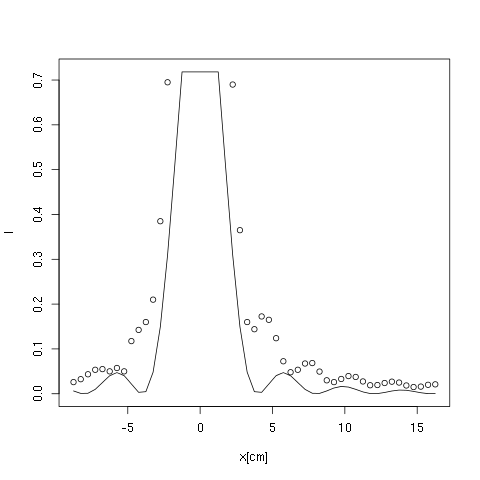
\includegraphics{wykres.png}

\end{document}
